\subsection{Analysis of Error Codes - OTG-ERR-001}
\subsubsection{BANK-APP}
\begin{longtable}{ p{2.3cm} | p{.79\linewidth} }\hline
    & \textbf{BANK-APP}
    \hfill CVSS Score: 4.3 \progressbar[filledcolor=BurntOrange]{0.43}
    \\ \hline
    \textbf{Observation} & 
    	Error messages:
    	\begin{itemize}
		  \item \textbf{Web server error Messages:} The Server runs Apache 2.2.22 on Ubuntu. The hostname of the server seems to be \enquote{samurai-wtf.localhost}
		  \item \textbf{Application Errors:} 
		  	\begin{itemize}
			  \item The Application uses Mysql constraints to check for duplicate Email addresses
			  \item Direct Mysql errors can be provoked when missusing the transaction html form
			  \item The Application presents the shell exit code in an error message in the transaction upload form
			\end{itemize}
		  \item Other Application errors do not contain valuable information
		\end{itemize}
    \\
    \textbf{Discovery} &
    	\textbf{Web server error Messages:}\newline
    	We used ErrorMint (see Fig.~\ref{fig:OTG_ERR_001_1} and Fig.~\ref{fig:OTG_ERR_001_2})to scan for the web server error messages on the web servers base url. The outputs where all similar to this:
    \\ &
    	\begin{lstlisting}[language=HTML, basicstyle=\footnotesize]
		<!DOCTYPE html>
		<html>
		<head><title>404 Not Found</title></head>
		<body>
		    <h1>Not Found</h1>
		    <p>The requested URL /index95381.html 
			was not found on this server.</p>
		    <hr>
		    <address>Apache/2.2.22 (Ubuntu) Server 
		    at 192.168.178.76 Port 80</address>
		</body>
		</html>
    	\end{lstlisting}
    	The 408 timeout message additionally provides \enquote{samurai-wtf.localhost} as host.
    	The html contains a hint to the used operating system and apache version.\newline
    	\textbf{Mysql constraints:}\newline
    	Using this curl command twice (remove newline caracters):
    	\begin{lstlisting}
    		curl 'http://192.168.178.76/secure-coding/public/
    		register.php'
			-H 'Content-Type: application/x-www-form-urlencoded'
			-H 'Connection: keep-alive' --data '
				firstname=Test&
				lastname=Test
				&email=example%40example.com
				&usertype=C&password=asd
				&confirm_password=asd&submit=
			' --compressed
    	\end{lstlisting}
    	result in following error:
    	\begin{lstlisting}
    	Duplicate entry 'example@example.com' for key 
    	'EMAIL_UNIQUE'
    	\end{lstlisting}
    \\ &
    	\textbf{Direct Mysql errors}\newline
    		See OTG-INPVAL-005\newline
    	\textbf{Shell exit code:}\newline
    		See OTG-INPVAL-013
    \\
    \textbf{Likelihood} &
    	An Atacker can use the informations presented by the error messages to validate further atacks. This results in a higher likelihood for other atacks.
    \\
    \textbf{Impact} & 
    	The Mysql errors can be used by an atacker to directly verify the success of his actions and help him to correct errors.
    	The Shell exit code error can help an atacker to retrieve viable information about the system if he manages to inject a command anywhere.
    \\
    \textbf{Recommen\-dations} &
        Hide the direct errors and transalte them to more general custom error messages.
    \\ \hline
    \textbf{CVSS} &
        \begin{tabular}[t]{@{}l | l}
            Attack Vector           & \textcolor{red}{Network} \\
            Attack Complexity       & \textcolor{red}{Low} \\
            Privileges Required     & \textcolor{BurntOrange}{Low} \\
            User Interaction        & \textcolor{red}{None} \\
            Scope                   & \textcolor{Green}{Unchanged} \\
            Confidentiality Impact  & \textcolor{BurntOrange}{Low} \\
            Integrity Impact        & \textcolor{Green}{None} \\
            Availability Impact     & \textcolor{Green}{None}
        \end{tabular}
    \\ \hline
\end{longtable}
\clearpage

\subsubsection{SecureBank}
\begin{longtable}{ p{2.3cm} | p{.79\linewidth} }\hline
    & \textbf{SecureBank}
    \hfill CVSS Score: 0 \progressbar{0}
    \\ \hline
    \textbf{Observation} & 
    	Error messages:
    	\begin{itemize}
		  \item \textbf{Web server error Messages:} The Server runs Apache 2.2.22 on Ubuntu.  The hostname of the server seems to be \enquote{samurai-wtf.localhost}. Instead of 404 an empty page with the letters \enquote{404} is returned. This is evidence that there is a php routing module involved.
		  \item \textbf{Application Errors:} 
		  	\begin{itemize}
			  \item The Application outputs a php exception with stack trace if a page is accessed unauthorized. See~\ref{fig:OTG_ERR_001_3}.
			\end{itemize}
			\item Other Application errors do not contain valuable information
		\end{itemize}
    \\
    \textbf{Discovery} &
    	\textbf{Web server error Messages:}\newline
    	See above. \newline
    	\textbf{Application Errors:}  \newline
    	See OTG-AUTHN-004.
    \\
    \textbf{Likelihood} & 
    	An Atacker can use the informations presented by the error messages to validate further atacks. This results in a higher likelihood for other atacks.
    \\
    \textbf{Impact} & 
    	An atacker can use the application errors to estimate application internas like file and include structures. The knowledge that there is a router involved can lead to specific atacks for routing components.
    \\
    \textbf{Recommen\-dations} &
        Hide the direct errors and transalte them to more general custom error messages.
    \\ \hline
    \textbf{CVSS} &
        \begin{tabular}[t]{@{}l | l}
            Attack Vector           & \textcolor{red}{Network} \\
            Attack Complexity       & \textcolor{red}{Low} \\
            Privileges Required     & \textcolor{red}{None} \\
            User Interaction        & \textcolor{red}{None} \\
            Scope                   & \textcolor{Green}{Unchanged} \\
            Confidentiality Impact  & \textcolor{Green}{None} \\
            Integrity Impact        & \textcolor{Green}{None} \\
            Availability Impact     & \textcolor{Green}{None}
        \end{tabular}
    \\ \hline
\end{longtable}

\subsubsection{Comparison}
While some of BANK-APPs error messages contian direct feedback of the success of an attack, SecureBank only discloses a bit of its internal structure.
\begin{figure}[p]
    \centering
    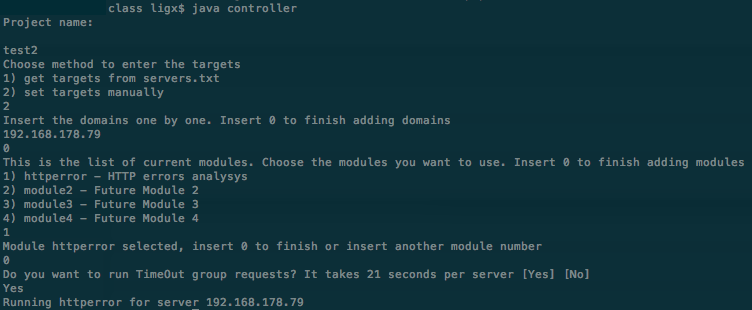
\includegraphics[width=0.8\textwidth]{figures/OTG-ERR-001-1.png}
    \caption{Usage of ErrorMint for SecureBank}
    \label{fig:OTG_ERR_001_1}
\end{figure}
\begin{figure}[p]
    \centering
    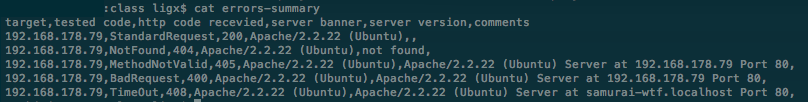
\includegraphics[width=0.8\textwidth]{figures/OTG-ERR-001-2.png}
    \caption{Output of ErrorMint for SecureBank}
    \label{fig:OTG_ERR_001_2}
\end{figure}
\begin{figure}[p]
    \centering
    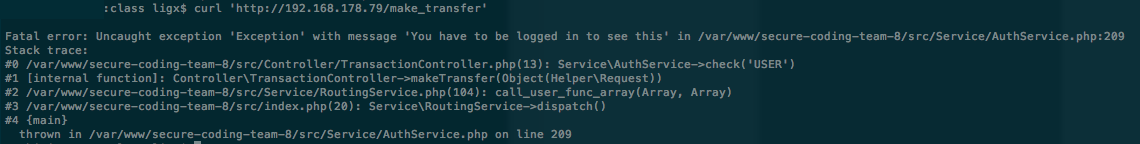
\includegraphics[width=0.8\textwidth]{figures/OTG-ERR-001-3.png}
    \caption{Stack trace when a page is accessed with no authorization in SecureBank}
    \label{fig:OTG_ERR_001_3}
\end{figure}
\clearpage